% This is text associated with the open textbook "Open Electromagnetics"
% See immediately below for author, date
% This work is licensed under the Creative Commons Attribution-ShareAlike 4.0 International License. (CC BY-SA 4.0) 
% To view a copy of the license, visit http://creativecommons.org/licenses/by-sa/4.0/

%ORB TITLE Plane Waves at Oblique Incidence on a Planar Boundary: TM Case
%ORB AUTHOR 0        # S.W. Ellingson, Virginia Tech (ellingson@vt.edu)
%ORB DATE 20191119   # yyyymmdd
%ORB ABSTRACT 

\label{m0164_Oblique_Incidence_TM} % <-- Must match name of this file and module directory name.  Don't mess with this!
\index{transverse magnetic|(}

In this section, we consider the problem of reflection and transmission from a planar boundary between semi-infinite media for a transverse magnetic (TM) uniform plane wave.
Before attempting this section, a review of
Sections~\ref{m0161_Waves_at_Planar_Boundary} (``Plane Waves at Normal Incidence on a Planar Boundary Between Lossless Media'') and
\ref{m0166_Decomposition_into_TE_and_TM} (``Decomposition of a Wave into TE and TM Components'') is recommended.
Also, note that this section has much in common with Section~\ref{m0167_Oblique_Incidence_TE} (``Plane Waves at Oblique Incidence on a Planar Boundary: TE Case''), and it is recommended to attempt the TE case first.

In this section, we consider the scenario illustrated in Figure~\ref{m0164_fObliqueTM}.
%
\begin{figure}[b!]
\begin{center}
\pdftooltip{{  % note double braces
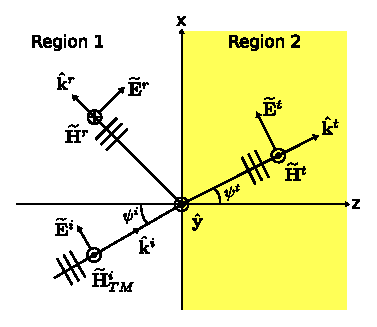
\includegraphics[width=0.8\columnwidth]{modules/m0164_fObliqueTM.eps} 
% https://commons.wikimedia.org/wiki/File:TM-polarized_upw_incident_on_planar_boundary.svg
}}{Transverse magnetic plane wave obliquely incident on a planar boundary. Magnetic field intensity out of page for incident wave and into page for reflected wave.}
\end{center}
\centerline{\scriptsize 
\copyright~\hyperref[m0164_fObliqueTM_Credit]{C.\ Wang} 
\href{https://creativecommons.org/licenses/by-sa/4.0/}{CC BY-SA 4.0} 
} 
\caption{
\label{m0164_fObliqueTM}
A TM uniform plane wave obliquely incident on the planar boundary between two semi-infinite material regions.
}
\end{figure}
%
The boundary between the two semi-infinite and lossless regions is located at the $z=0$ plane.
The wave is incident from Region~1. 
The magnetic field intensity $\widetilde{\bf H}^i_{TM}$ of this wave is given by
%
\begin{equation}
\widetilde{\bf H}^i_{TM}({\bf r}) = \hat{\bf y} H^i_{TM} e^{-j{\bf k}^i\cdot{\bf r}}
\label{m0164_eHi}
\end{equation}
%
In this expression, ${\bf r}$ is the position at which $\widetilde{\bf H}^i_{TM}$ is evaluated.
Also,
%
\begin{equation}
{\bf k}^i = \hat{\bf k}^i \beta_1
\end{equation}
%
where
$\hat{\bf k}^i$ is the unit vector indicating the direction of propagation and
$\beta_1=\omega\sqrt{\mu_1 \epsilon_1}$ is the phase propagation constant in Region~1. 
$\widetilde{\bf H}^i_{TM}$ serves as the ``stimulus'' in this problem, and all other contributions to the total field may be expressed in terms of parameters associated with Equation~\ref{m0164_eHi}.

The presence of reflected and transmitted uniform plane waves is inferred from our experience with the normal incidence scenario (Section~\ref{m0161_Waves_at_Planar_Boundary}).
There, as here, the symmetry of the problem indicates that the reflected and transmitted components of the magnetic field will have the same polarization as that of the incident electric field.  This is because there is nothing present in the problem that could account for a change in polarization.
Thus, the reflected and transmitted fields will also be TM.
So we postulate the following expression for the reflected wave:
%
\begin{equation}
\widetilde{\bf H}^r({\bf r}) = -\hat{\bf y} B e^{-j{\bf k}^r\cdot{\bf r}}
\label{m0164_eHr}
\end{equation}
%
where $B$ is an unknown, possibly complex-valued constant to be determined and
%
\begin{equation}
{\bf k}^r = \hat{\bf k}^r \beta_1
\end{equation}
%
indicates the direction of propagation. 

The reader may wonder why we have chosen $-\hat{\bf y}$, as opposed to $+\hat{\bf y}$, as the reference polarization for $\widetilde{\bf H}^r$.
In fact, either $+\hat{\bf y}$ or $-\hat{\bf y}$ could be used.
However, the choice is important because the form of the results we obtain in this section -- specifically, the reflection coefficient -- will be determined with respect to this specific convention, and will be incorrect with respect to the opposite convention.
We choose $-\hat{\bf y}$ because it has a particular advantage which we shall point out at the end of this section.

Continuing, we postulate the following expression for the transmitted wave:
%
\begin{equation}
\widetilde{\bf H}^t({\bf r}) = \hat{\bf y} C e^{-j{\bf k}^t\cdot{\bf r}}
\label{m0164_eHt}
\end{equation}
%
where $C$ is an unknown, possibly complex-valued constant to be determined and
%
\begin{equation}
{\bf k}^t = \hat{\bf k}^t \beta_2
\end{equation}
%
where
$\hat{\bf k}^t$ is the unit vector indicating the direction of propagation and
$\beta_2=\omega\sqrt{\mu_2 \epsilon_2}$ is the phase propagation constant in Region~2.

At this point, the unknowns in this problem are the constants $B$ and $C$, as well as the unknown directions $\hat{\bf k}^r$ and $\hat{\bf k}^t$.  
We may establish a relationship between $H^i_{TM}$, $B$, and $C$ by application of boundary conditions at $z=0$.  
First, we presume no impressed current at the boundary.
Thus, the tangential component of the total magnetic field intensity must be continuous across the boundary.
To apply this boundary condition, let us define $\widetilde{\bf H}_1$ and $\widetilde{\bf H}_2$ to be the total magnetic fields in Regions~1 and 2, respectively.
The total field in Region~1 is the sum of incident and reflected fields, so
%
\begin{equation}
\widetilde{\bf H}_1({\bf r}) = \widetilde{\bf H}^i_{TM}({\bf r}) + \widetilde{\bf H}^r({\bf r})
\end{equation}
%
The field in Region~2 is simply
%
\begin{equation}
\widetilde{\bf H}_2({\bf r}) = \widetilde{\bf H}^t({\bf r})
\end{equation}
%
Also, we note that all magnetic field components are already tangent to the boundary.
Thus, continuity of the tangential component of the magnetic field across the boundary requires $\widetilde{\bf H}_1({\bf r}_0)=\widetilde{\bf H}_2({\bf r}_0)$,  
where ${\bf r}_0\triangleq\hat{\bf x}x+\hat{\bf y}y$ since $z=0$ on the boundary.
Therefore,
%
\begin{equation}
\widetilde{\bf H}^i_{TM}({\bf r}_0) + \widetilde{\bf H}^r({\bf r}_0)  = \widetilde{\bf H}^t({\bf r}_0) 
\end{equation}
%
Now employing Equations~\ref{m0164_eHi}, \ref{m0164_eHr}, and \ref{m0164_eHt}, we obtain:
%
\begin{equation}
\hat{\bf y}H^i_{TM}e^{-j{\bf k}^i\cdot{\bf r}_0} - 
\hat{\bf y}B         e^{-j{\bf k}^r\cdot{\bf r}_0} = 
\hat{\bf y}C         e^{-j{\bf k}^t\cdot{\bf r}_0}
\label{m0164_eBCH}
\end{equation}
%
Dropping the vector ($\hat{\bf y}$) since it is the same in each term, we obtain:
%
\begin{equation}
H^i_{TM}e^{-j{\bf k}^i\cdot{\bf r}_0} - 
B         e^{-j{\bf k}^r\cdot{\bf r}_0} = 
C         e^{-j{\bf k}^t\cdot{\bf r}_0}
\label{m0164_eBCH2}
\end{equation}
%
For this to be true at every point ${\bf r}_0$ on the boundary, it must be true that
%
\begin{equation}
{\bf k}^i\cdot{\bf r}_0 = {\bf k}^r\cdot{\bf r}_0 = {\bf k}^t\cdot{\bf r}_0
\label{m0164_eSL}
\end{equation}
%
%
Essentially, we are requiring the phases of each field in Regions~1 and 2 to be matched at every point along the boundary.
Any other choice will result in a violation of boundary conditions at some point along the boundary.
This expression allows us to solve for the directions of propagation of the reflected and transmitted fields, which we shall do later.  
Our priority for now shall be to solve for the coefficients $B$ and $C$. 

Enforcing Equation~\ref{m0164_eSL}, we observe that Equation~\ref{m0164_eBCH2} reduces to:
%
\begin{equation}
H^i_{TM} - B = C 
\label{m0164_eBCH3}
\end{equation}

A second equation is needed since we currently have only one equation (Equation~\ref{m0164_eBCH3}) and two unknowns ($B$ and $C$).  
The second equation is obtained by applying the appropriate boundary conditions to the electric field.
The electric field associated with each of the magnetic field components is identified in Figure~\ref{m0164_fObliqueTM}.
Note the orientations of the electric field vectors may be confirmed using the \emph{plane wave relationships}: 
\index{plane wave relationships}
Specifically, the cross product of the electric and magnetic fields should point in the direction of propagation.
Expressions for each of the electric field components is determined formally below.

From the plane wave relationships, we determine that the incident electric field intensity is
%
\begin{equation}
\widetilde{\bf E}^i({\bf r}) = -\eta_1 \hat{\bf k}^i \times \widetilde{\bf H}^i_{TM}              
\label{m0164_eEi}
\end{equation}
%
where $\eta_1=\sqrt{\mu_1 / \epsilon_1}$ is the wave impedance in Region~1.  
%
To make progress requires that we express $\hat{\bf k}^i$ in the global fixed coordinate system.  Here it is:
%
\begin{equation}
\hat{\bf k}^i = \hat{\bf x}\sin\psi^i + \hat{\bf z}\cos\psi^i 
\end{equation}
%
Thus:
%
\begin{equation}
\widetilde{\bf E}^i({\bf r}) = \left( \hat{\bf x}\cos\psi^i - \hat{\bf z}\sin\psi^i \right) \eta_1 H^i_{TM}  e^{-j{\bf k}^i\cdot{\bf r}}          
\label{m0164_eEi2}
\end{equation}
%
Similarly we determine that the reflected electric field has the form:
%
\begin{equation}
\widetilde{\bf E}^r({\bf r}) = -\eta_1 \hat{\bf k}^r \times \widetilde{\bf H}^r              
\label{m0164_eEr}
\end{equation}
%
In the global coordinate system:
%
\begin{equation}
\hat{\bf k}^r = \hat{\bf x}\sin\psi^r - \hat{\bf z}\cos\psi^r 
\label{m0164_ehkr}
\end{equation}
%
Thus:
%
\begin{equation}
\widetilde{\bf E}^r({\bf r}) = \left( \hat{\bf x}\cos\psi^r + \hat{\bf z}\sin\psi^r \right) \eta_1 B  e^{-j{\bf k}^r\cdot{\bf r}}          
\label{m0164_eEr2}
\end{equation}
%
The transmitted magnetic field has the form:
%
\begin{equation}
\widetilde{\bf E}^t({\bf r}) = -\eta_2 \hat{\bf k}^t \times \widetilde{\bf H}^t              
\label{m0164_eEt}
\end{equation}
%
In the global coordinate system:
%
\begin{equation}
\hat{\bf k}^t = \hat{\bf x}\sin\psi^t + \hat{\bf z}\cos\psi^t 
\label{m0164_ehkt}
\end{equation}
%
Thus:
%
\begin{equation}
\widetilde{\bf E}^t({\bf r}) = \left( \hat{\bf x}\cos\psi^t - \hat{\bf z}\sin\psi^t \right) \eta_2 C  e^{-j{\bf k}^t\cdot{\bf r}}          
\label{m0164_eEt2}
\end{equation}
%
The total electric field in Region~1 is the sum of incident and reflected fields, so
%
\begin{equation}
\widetilde{\bf E}_1({\bf r}) = \widetilde{\bf E}^i({\bf r}) + \widetilde{\bf E}^r({\bf r})
\end{equation}
%
The electric field in Region~2 is simply
%
\begin{equation}
\widetilde{\bf E}_2({\bf r}) = \widetilde{\bf E}^t({\bf r})
\end{equation}
%
The tangential component of the total electric field intensity must be continuous across the boundary.
Expressed in terms of the quantities already established, this boundary condition requires:
%
\begin{equation}
\hat{\bf x}\cdot\widetilde{\bf E}^i({\bf r}_0) + \hat{\bf x}\cdot\widetilde{\bf E}^r({\bf r}_0)  = \hat{\bf x}\cdot\widetilde{\bf E}^t({\bf r}_0) 
\end{equation}
%
where ``$\hat{\bf x}\cdot$'' selects the component of the electric field that is tangent to the boundary.
Evaluating this expression, we obtain:
%
\begin{flalign}
  &+\left(\cos\psi^i\right) \eta_1 H^i_{TM} e^{-j{\bf k}^i\cdot{\bf r}_0} \nonumber \\
  &+\left(\cos\psi^r\right) \eta_1 B e^{-j{\bf k}^r\cdot{\bf r}_0} \nonumber \\
= &+\left(\cos\psi^t\right) \eta_2 C e^{-j{\bf k}^t\cdot{\bf r}_0} 
\end{flalign}
%
Now employing the ``phase matching'' condition expressed in Equation~\ref{m0164_eSL}, we find:
%
\begin{flalign}
  &+\left(\cos\psi^i\right) \eta_1 H^i_{TM} \nonumber \\
  &+\left(\cos\psi^r\right) \eta_1 B \nonumber \\
= &+\left(\cos\psi^t\right) \eta_2 C 
\label{m0164_eBCE3}
\end{flalign}

Equations~\ref{m0164_eBCH3} and \ref{m0164_eBCE3} comprise a linear system of equations with unknowns $B$ and $C$.
This system of equations is easily solved for $B$ as follows.
First, use Equation~\ref{m0164_eBCH3} to eliminate $C$ in Equation~\ref{m0164_eBCE3}.
The result is: 
%
\begin{flalign}
  &+\left(\cos\psi^i\right) \eta_1 H^i_{TM} \nonumber \\
  &+\left(\cos\psi^r\right) \eta_1 B \nonumber \\
= &+\left(\cos\psi^t\right) \eta_2 \left( H^i_{TM} - B \right)
\end{flalign}
%
Solving this equation for $B$, we obtain:
%
\begin{equation}
B = \frac{-\eta_1\cos\psi^i+\eta_2\cos\psi^t}{+\eta_1\cos\psi^r+\eta_2\cos\psi^t} ~ H^i_{TM}
\end{equation}
%
We can express this result as follows:
%
\begin{equation}
B = \Gamma_{TM} H^i_{TM} 
\end{equation}
%
where we have made the definition
%
\begin{equation}
\Gamma_{TM} \triangleq \frac{-\eta_1\cos\psi^i+\eta_2\cos\psi^t}{+\eta_1\cos\psi^r+\eta_2\cos\psi^t}
\label{m0164_eGTM}
\end{equation}

We are now able to express the complete solution in terms of the electric field intensity.
First we make the substitution $E^i_{TM} \triangleq \eta_1 H^i_{TM}$ in Equation~\ref{m0164_eEi2}, yielding:
%
\begin{equation}
\widetilde{\bf E}^i({\bf r}) = \left( \hat{\bf x}\cos\psi^i - \hat{\bf z}\sin\psi^i \right) E^i_{TM} e^{-j{\bf k}^i\cdot{\bf r}}          
\end{equation}
%
The factor $\eta_1 B$ in Equation~\ref{m0164_eEr2} becomes $\Gamma_{TM}E^i_{TM}$, so we obtain:
%
\begin{flalign}
\widetilde{\bf E}^r({\bf r}) = &\left( \hat{\bf x}\cos\psi^r + \hat{\bf z}\sin\psi^r \right) \nonumber \\
                               &\cdot\Gamma_{TM} E^i_{TM} e^{-j{\bf k}^r\cdot{\bf r}}          
\end{flalign}
%
Thus, we see $\Gamma_{TM}$ is the reflection coefficient for the electric field intensity.

Returning to Equation~\ref{m0164_eBCH3}, we now find
%
\begin{flalign}
C &= H^i_{TM}-B \nonumber \\
  &= H^i_{TM}-\Gamma_{TM} H^i_{TM} \nonumber \\
  &= \left(1-\Gamma_{TM}\right) H^i_{TM} \nonumber \\
  &= \left(1-\Gamma_{TM}\right) E^i_{TM}/\eta_1
\end{flalign}
%
Subsequently, Equation~\ref{m0164_eEt2} becomes
%
\begin{flalign}
\widetilde{\bf E}^t({\bf r}) = &\left( \hat{\bf x}\cos\psi^t - \hat{\bf z}\sin\psi^t \right) \nonumber \\
                               &\cdot \left(1-\Gamma_{TM}\right) \frac{\eta_2}{\eta_1} E^i_{TM} e^{-j{\bf k}^t\cdot{\bf r}}          
\end{flalign}

This solution is complete except that we have not yet determined 
$\hat{\bf k}^r$, which is now completely determined by $\psi^r$ via Equation~\ref{m0164_ehkr}, and
$\hat{\bf k}^t$, which is now completely determined by $\psi^t$ via Equation~\ref{m0164_ehkt}.
In other words, we have not yet determined the directions of propagation 
$\psi^r$ for the reflected wave and
$\psi^t$ for the transmitted wave.
However, $\psi^r$ and $\psi^i$ can be found using Equation~\ref{m0164_eSL}.
Here we shall simply state the result, and in Section~\ref{m0168_Angles_of_Reflection_and_Refraction} we shall perform this part of the derivation in detail and with greater attention to the implications.
One finds:
%
\begin{equation}
\psi^r = \psi^i
\label{m0164_epsir}
\end{equation}
%
i.e., angle of reflection equals angle of incidence.
Also, 
%
\begin{equation}
\psi^t = \arcsin\left(\frac{\beta_1}{\beta_2}\sin\psi^i\right)
\label{m0164_epsit}
\end{equation}
%
Astute readers may notice that there is something fishy about Equation~\ref{m0164_epsit}.
Namely, it seems possible for the argument of $\arcsin$ to be greater than one.
This oddity is addressed in Section~\ref{m0168_Angles_of_Reflection_and_Refraction}.

Now let us return to the following question, raised near the beginning of this section:  
Why choose $-\hat{\bf y}$, as opposed to $+\hat{\bf y}$, as the reference polarization for ${\bf H}^r$, as shown in Figure~\ref{m0164_fObliqueTM}?
To answer this question, first note that $\Gamma_{TM}$ (Equation~\ref{m0164_eGTM}) becomes the reflection coefficient for normal (TEM) incidence when $\psi^i=\psi^t=0$.
If we had chosen $+\hat{\bf y}$ as the reference polarization for ${\bf H}^r$, we would have instead obtained an expression for $\Gamma_{TM}$ that has the opposite sign for TEM incidence.\footnote{Obtaining this result is an excellent way for the student to confirm their understanding of the derivation presented in this section.}
There is nothing wrong with this answer, but it is awkward to have different values of the reflection coefficient for the same physical scenario.
By choosing $-\hat{\bf y}$, the reflection coefficient for the oblique incidence case computed for $\psi^i=0$ converges to the reflection coefficient previously computed for the normal-incidence case.
It is important to be aware of this issue, as one occasionally encounters work in which the opposite (``$+\hat{\bf y}$'') reference polarization has been employed.

Finally, note that Equation~\ref{m0164_epsir} allows us to eliminate $\psi^r$ from Equation~\ref{m0164_eGTM}, yielding:
%
\begin{equation}
\boxed{
\Gamma_{TM} = \frac{-\eta_1\cos\psi^i+\eta_2\cos\psi^t}{+\eta_1\cos\psi^i+\eta_2\cos\psi^t}
}
\label{m0164_eGTM2}
\end{equation}
Thus, we obtain what is perhaps the most important finding of this section:
%%%%%%%%%%%%%%%%%%%%%%%%%%%%%%%%%%%%%%%%%%%%%%%
%ORB HIGHLIGHT
\begin{mdframed}[backgroundcolor=yellow!20,nobreak=true] 
The electric field reflection coefficient for oblique TM incidence, $\Gamma_{TM}$, is given by Equation~\ref{m0164_eGTM2}.
\end{mdframed}
%%%%%%%%%%%%%%%%%%%%%%%%%%%%%%%%%%%%%%%%%%%%%%%
The following example demonstrates the utility of this result.

%%%%%%%%%%%%%%%%%%%%%%%%%%%%%%%%%%%%%%%%%%%%%%%
%ORB EXAMPLE
~\\ \begin{example} 
\begin{mdframed}[backgroundcolor=brown!20,linecolor=brown!20]\raggedright
Power transmission at an air-to-glass interface (TM case).
\\~\\
Figure~\ref{m0164_fGlassExample} illustrates a TM plane wave incident from air onto the planar boundary with a glass region.
The glass exhibits relative permittivity of 2.1.  
Determine the power reflected and transmitted relative to power incident on the boundary.\\
~\\

\noindent
{\bf Solution.}
The power reflected relative to power incident is $\left|\Gamma_{TM}\right|^2$ whereas
the power transmitted relative to power incident is $1-\left|\Gamma_{TM}\right|^2$.
$\Gamma_{TM}$ may be calculated using Equation~\ref{m0164_eGTM2}.
Calculating the quantities that enter into this expression:
%
\begin{equation} 
\eta_1 \approx \eta_0 \cong 376.7~\Omega ~~ \mbox{(air)} 
\end{equation}
%
\begin{equation} 
\eta_2 \approx \frac{\eta_0}{\sqrt{2.1}} \cong 260.0~\Omega ~~ \mbox{(glass)}
\end{equation}
%
\begin{equation} 
\psi^i = 30^{\circ} 
\end{equation}
Note
%
\begin{equation} 
\frac{\beta_1}{\beta_2} \approx \frac{\omega\sqrt{\mu_0\epsilon_0}}{\omega\sqrt{\mu_0\cdot2.1\epsilon_0}} \cong 0.690 
\end{equation}
so
%
\begin{equation} 
\psi^t = \arcsin\left(\frac{\beta_1}{\beta_2}\sin\psi^i\right) \cong 20.2^{\circ} 
\end{equation}
%
Now substituting these values into Equation~\ref{m0164_eGTM2}, we obtain
%
\begin{equation} 
\Gamma_{TM} \cong -0.1442 
\end{equation}
(Did you get an answer closer to $-0.1323$? If so, you probably did not use sufficient precision to represent intermediate results.  This is a good example of a problem in which three significant figures for results that are used in subsequent calculations is not sufficient.)

\noindent
The fraction of power reflected relative to power incident is now determined to be $\left|\Gamma_{TM}\right|^2\cong 0.021$; i.e., about \underline{2.1\%}.
$1-\left|\Gamma_{TM}\right|^2\cong$ \underline{97.9\%} of the power is transmitted into the glass.
\end{mdframed}
%
\begin{figure}
\begin{center}
\pdftooltip{{  % note double braces
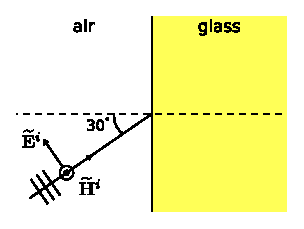
\includegraphics[width=0.8\columnwidth]{modules/m0164_fGlassExample.eps} 
% https://commons.wikimedia.org/wiki/File:TM-polarized_upw_incident_from_air_to_glass.svg
}}{Transverse magnetic uniform plane wave incident on the planar boundary between two media. Magnetic field intensity out of page and electric field perpendicular to incident wave.}
\end{center}
\centerline{\scriptsize 
\copyright~\hyperref[m0164_fGlassExample_Credit]{C.\ Wang} 
\href{https://creativecommons.org/licenses/by-sa/4.0/}{CC BY-SA 4.0} 
} 
\caption{
\label{m0164_fGlassExample}
A TM uniform plane wave incident from air to glass.
}
\end{figure}
\end{example}
%%%%%%%%%%%%%%%%%%%%%%%%%%%%%%%%%%%%%%%%%%%%%%%

Note that the result obtained in the preceding example is different from the result for a TE wave incident from the same direction (Example~\ref{m0167_exTERC}). 
In other words:
%
%%%%%%%%%%%%%%%%%%%%%%%%%%%%%%%%%%%%%%%%%%%%%%%
%ORB HIGHLIGHT
\begin{mdframed}[backgroundcolor=yellow!20,nobreak=true] 
The fraction of power reflected and transmitted from the planar boundary between dissimilar media depends on the polarization of the incident wave relative to the boundary, as well as the angle of incidence.
\end{mdframed}
%%%%%%%%%%%%%%%%%%%%%%%%%%%%%%%%%%%%%%%%%%%%%%%

\index{transverse magnetic|)}


